\subsection{圆柱体等三维图形的绘制}

%% 核心思想还是三维图形的二维坐标化
\begin{example}
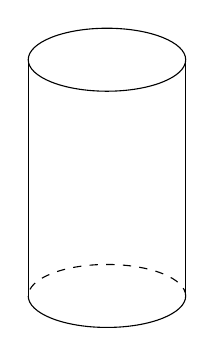
\begin{tikzpicture}
\draw (-1, 0) -- (-1, 3);
\draw (1,0) -- (1, 3);

%% 绘制椭圆
\draw (0, 3) ellipse [x radius=1, y radius=0.4];
% \draw (0, 0) ellipse [x radius=1, y radius=0.4];
\draw[dashed] (1, 0) arc [start angle=0, 
                          end angle=180, 
                          x radius=1, 
                          y radius=0.4];
\draw (1, 0) arc [start angle=0, 
                  end angle=-180, 
                  x radius=1, 
                  y radius=0.4];
\end{tikzpicture}    
\end{example}
